%--------|---------|---------|---------|---------|---------|---------|---------|
%       10        20        30        40        50        60        70        80
%-------------------------------------------------------------------------------



\documentclass[11pt, twoside, titlepage, a4paper]{article}
% set utf8 encoding, and set font encoding T1 to allow "|" ">" "<" etc
\usepackage[utf8]{inputenc}
\usepackage[T1]{fontenc}
\usepackage[a4paper,inner=40mm,outer=25mm,top=25mm,bottom=25mm,pdftex]{geometry}
% These page settings give images 1.0\linewidth around 135-140mm wide (ca 138mm)
% meaning a 300dpi image is around 1600 pixels wide
\usepackage{graphicx}   % For eps figures
\usepackage{epsfig}     % Alternative package
\usepackage[hang,small,bf]{caption}

\usepackage[british]{babel}       

\usepackage[yyyymmdd]{datetime}
\renewcommand{\dateseparator}{--}

\usepackage{fancyhdr}
\pagestyle{fancy}
% with this we ensure that the chapter and section
% headings are in lowercase.
%\renewcommand{\chaptermark}[1]{\markboth{#1}{}}  % no "\chapter" in article doc type
\renewcommand{\sectionmark}[1]{\markright{\thesection\ #1}}
\fancyhf{} % delete current setting for header and footer
\fancyhead[LE,RO]{\bfseries\thepage}
\fancyhead[LO]{\bfseries\rightmark}
\fancyhead[RE]{\bfseries\leftmark}
\renewcommand{\headrulewidth}{0.5pt}
\renewcommand{\footrulewidth}{0pt}
\addtolength{\headheight}{0.5pt} % make space for the rule
\fancypagestyle{plain}{%
    \fancyhead{} % get rid of headers on plain pages
    \renewcommand{\headrulewidth}{0pt} % and the line
}


% remove forced implicit vertical whitespace before and after verbatim environment
\makeatletter
\preto{\@verbatim}{\topsep=0pt \partopsep=0pt }
\makeatother


% allow to force indentation of first line in section
% \indent is not working, so workaround \hspace{\parindent} works
\newcommand{\forceindent}{\hspace{\parindent}}


\newcommand{\degrees}{$^\circ$~}
\newcommand{\degree}{$^\circ$}
\newcommand{\ca}{$\approx$}

\newcommand{\vs}{$\backslash\ $}  % "versus" slash
\newcommand{\bs}{$\backslash\ $}  % just backslash


% want clear dash insert commands
\newcommand{\dash}{-}     % just a normal hyphen dash  "-"
\newcommand{\ndash}{--}   % n-dash "--"
\newcommand{\mdash}{---}  % m-dash "---"


%link new command names to the original font sizes,
%for easier to remember smaller font size
\newcommand{\vsmall}{\footnotesize}  % simpler to remember
\newcommand{\vvsmall}{\scriptsize}   %
%\newcommand{\vvvsmall}{\tiny}


\usepackage[colorlinks=true,linkcolor=black,urlcolor=blue]{hyperref}


\usepackage{ifthen}


% \needspace{5\baselineskip}      << reserves approximately 5 lines, leaves raggedbottom, more efficient
% \Needspace{5\baselineskip}      << reserves exactly 5 lines, leaves raggedbottom, less efficient
% \Needpsace*{5\baselineskip}     << leaves flushbottom if \flushbottom is in effect, otherwise ragged
\usepackage{needspace}



% \skill{blabla}
\newboolean{skillsaslist}
\setboolean{skillsaslist}{true}
\ifthenelse{\boolean{skillsaslist}}{\newcommand{\skill}[1]{\item[#1]}}{\newcommand{\skill}[1]{\subsubsection*{#1}}}
\ifthenelse{\boolean{skillsaslist}}{\newcommand{\openskillslist}{\begin{description}}}{\newcommand{\openskillslist}{}}
\ifthenelse{\boolean{skillsaslist}}{\newcommand{\closeskillslist}{\end{description}}}{\newcommand{\closeskillslist}{}}

% \action{blabla}
\newboolean{actionsaslist}
\setboolean{actionsaslist}{true}
\ifthenelse{\boolean{actionsaslist}}{\newcommand{\action}[1]{\item[#1]}}{\newcommand{\action}[1]{\subsubsection*{#1}}}
\ifthenelse{\boolean{actionsaslist}}{\newcommand{\openactionslist}{\begin{description}}}{\newcommand{\openactionslist}{}}
\ifthenelse{\boolean{actionsaslist}}{\newcommand{\closeactionslist}{\end{description}}}{\newcommand{\closeactionslist}{}}

% \eqitem{blabla}
\newboolean{itemsaslist}
\setboolean{itemsaslist}{true}
\ifthenelse{\boolean{itemsaslist}}{\newcommand{\eqitem}[1]{\item[#1]}}{\newcommand{\eqitem}[1]{\subsubsection*{#1}}}
\ifthenelse{\boolean{itemsaslist}}{\newcommand{\openitemslist}{\begin{description}}}{\newcommand{\openactionslist}{}}
\ifthenelse{\boolean{itemsaslist}}{\newcommand{\closeitemslist}{\end{description}}}{\newcommand{\closeactionslist}{}}


\newenvironment{readoutloud}%
{\begin{quote}\begin{itshape}}%
{\end{itshape}\end{quote}}%



% need a nice easily visible TODO marker
\newcommand{\todo}{\textbf{TODO:}~}
\newcommand{\TODO}{\LARGE\textbf{TODO:}\normalsize~}






%-------------------------------------------------------------------------------
\begin{document}


% too many words in common across docs nowadays
%--------|---------|---------|---------|---------|---------|---------|---------|
%       10        20        30        40        50        60        70        80
%-------------------------------------------------------------------------------


% Manually specify hyphenation for names.
% Remember: space separated word list: lead with space
% hyphens can only occur on specified "-" characters
% words without "-" will never be hyphenated, overrides language rules
\hyphenation{
 cam-paign-ab-il-ity
 Thing-a-ma-jig
 milli-fort-night
 Kings-land
 Evil-nius Conq
 Massa Pawa
 Maj-san Go-san Mal-vi-na
 Ho-her
 Bea-ta Blo-dig
 Leg-io Legu-ano
 Gammel-Tant
 Gam-ling
 Hem-ske-lina
 Go-blan-da
 Stur-Skurk
 Hjal-mar Hjäl-te
 Bur-mak
 Lund-qvist
 Grim-Gnash
 Gros-Orc
 muta-mon-ster
 muta-meat
 Iffy-Griff
 Hoo-man Hoo-mans hoo-man hoo-mans
 Da-ta-ri-an Ma-ras No-stro-mo
 Uchly Namen
 Edwin Chro-mo-phobe
 Star-Craft Brood War Brood-War
 Space Hulk
 Hermann Hammer-hand
}




%-------------------------------------------------------------------------------
% title page
%-----------


\thispagestyle{empty}

\null          % make an empty mark, so that following white space will be honoured
\vspace{1cm}   % not honoured at beginning of page without something above

\begin{center}

\huge         Adventures  \\
                  in      \\
              Kingsland

\vspace{0.3\baselineskip}

\large      Gold and Glory

\vspace{2cm}

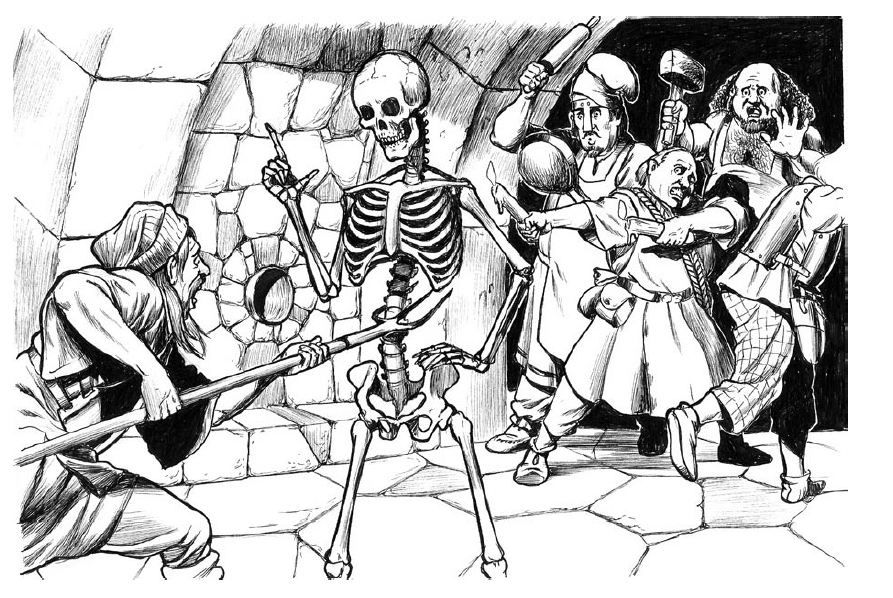
\includegraphics[width=120mm]{./fig/skeleton.jpg}

\vspace{2 cm}


\normalsize
          your guide to the local    \\
            corner of the world

\vfill

\today

\end{center}






%-------------------------------------------------------------------------------
% copyright etc on the back side of the title page
%-------------------------------------------------
\clearpage
\thispagestyle{empty}
\raggedbottom

\vsmall
\noindent
This work is licensed under a Creative Commons \\
Attribution-NonCommercial-ShareAlike 4.0 \\
International License. (CC BY-NC-SA 4.0).\\
\url{https://creativecommons.org/licenses/by-nc-sa/4.0/} \\
\url{https://creativecommons.org/licenses/by-nc-sa/4.0/legalcode} \\
If you want to use it in any other fashion please contact the author.

\

\noindent
All images are temporary placeholders, \\
most are downloaded and unattributed.\\
They need to be replaced with licensed art.

\normalsize






%-------------------------------------------------------------------------------
% begin main matter
%------------------
\cleardoublepage
\pagestyle{fancy}
%\flushbottom
\raggedbottom


% will mark both left and right pages with an abbreviated section title
% since this is most likely to be read on screens one page at a time instead of
% printed in a binder/book with left/right pages visible simultaneously.
%\markboth{lefttitle}{righttitle}




%--------|---------|---------|---------|---------|---------|---------|---------|
%       10        20        30        40        50        60        70        80
%-------------------------------------------------------------------------------
\section*{Adventures in Kingsland}
\markboth{Kingsland}{Kingsland}

\noindent
Play online with your bestest buddies, a couple of hours on weekday evenings, after the kids fall asleep, or from the hotel room when you're travelling for work. Easy to schedule, designed for virtual tabletop and voice chat.
Fast and tactically challenging tabletop battles, exciting adventures, tricky dungeon crawls, and mini war games, set in silly cliché role playing campaigns.
Build the optimal monster-murder squad, tinker with skills, weapons, magic, etc, for that special clever edge, or that over the top character which is a shitload of fun to play.

\

\emph{Or}

\

\noindent
Play with the kids on the dining room table, or across half the house. Use their favourite toys as Hero figs and the dreaded \textsc{lego} men as the countless minions of Lord Grapefruit.
Simple, quick, fun role playing adventures full of wonder, exploration, puzzles, riddles, and perhaps some tricksy fights if the GM is so inclined.
Huge width of freedom in character creation with a skill based, classless, rule set where you can choose the complexity level you want to find the sweet spot between fast simple fun and challenging depth and complexity.

\

\emph{You decide}

\

\noindent
The rule set is highly flexible. The basics is simple enough for very young kids. The full complete rule set leaves enough room for a clever scientist to tinker and get lost in.




\vfill

\begin{center}
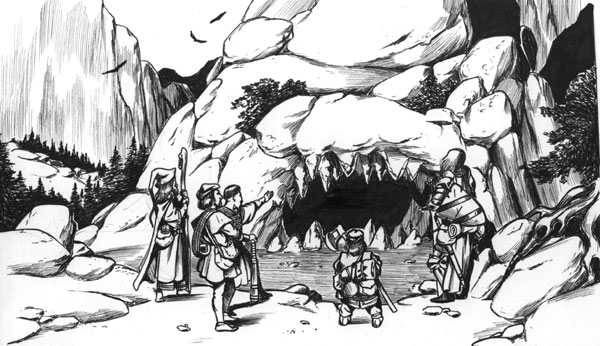
\includegraphics[width=120mm]{./fig/cavemouth.jpg}
\end{center}

\vfill




\noindent
Explicitly designed for fast online play. Easy to schedule for busy people. Small and simple basic rule set with inherent tactical depth and very quick play. Lots of optional addons for extra depth and complexity so you can choose your own game style.

This is not like D\&D, d20, Cypher, GURPS, Warhammer, WoD/Storyteller, Fate, Savage Worlds, et al. It is faster and with more tactical depth. Trading real world realism for speed and storytelling, coolness and heroics. Optimised for fast online play. The game is classless, skill based, and the skills directly change the rules of the game. It plays more like Space Hulk style fighting wrapped in fantasy adventure campaigns.







\clearpage %--------------------------------------------------------------------

\noindent
\section*{Why \emph{this} game?}

\noindent
Actually get to play! Gameplay is fast enough that an hour or two is still meaningful game time. Play online: No travel. Very quick to start up and get going. Weekday evenings, a couple of hours, works for most people. Easy to schedule!

\

\noindent
Tactical depth, interesting fights, huge build and optimisation space. The core design is small, flexible, classless, skill based, and the skills directly change game rules.

Fast gameplay improves depth. With many short rounds the fights are fluid. Scout, plan, sneak, attack, retreat, move and reposition, traps and tricks, regroup, hold, flank, map control, and changing combat goals.
Battles have a dynamic feel more like StarCraft Brood War and goal progression like Space Hulk missions. No static dice rally.

You can't just pour a bucket of attack dice on a monster. You'll just end up dead and wondering why. Think, observe, adapt, outsmart. Find ways around defences.

\

\noindent
Simple or wildly complex, with meaningful interactions but few interdependencies. You can very easily tailor the game to your preferences. Speed vs complexity, simplicity vs variation, and the relationships are much better than linear. The primary depth comes from the tiny core design itself. Optional addons expands the game and interact in interesting ways. Pick what you like and skip the rest. Lots of options.

I built the game for myself and my players, most of which are engineers or scientists. The fact that it scales down very well for young kids is a wonderful bonus, and a product of the design principles. Same for physical tabletop gaming.

\

\noindent
Some basic ideas form the core design: Trade real world realism for fun, fast, flexible, interesting, and deep game play. But keep internal consistency and verisimilitude, which are crucial for long term enjoyment.

Scouting, information gathering, coordination, movement, positioning, understanding the opponent, adapting your fighting style to the moment. All crucial elements here, but rare in games today. Different weapons have very distinct feel and behaviour, and require different tactics to use. It's not just a bit of a damage difference and some special ability thingy you can use once per day.





\vfill

\begin{center}
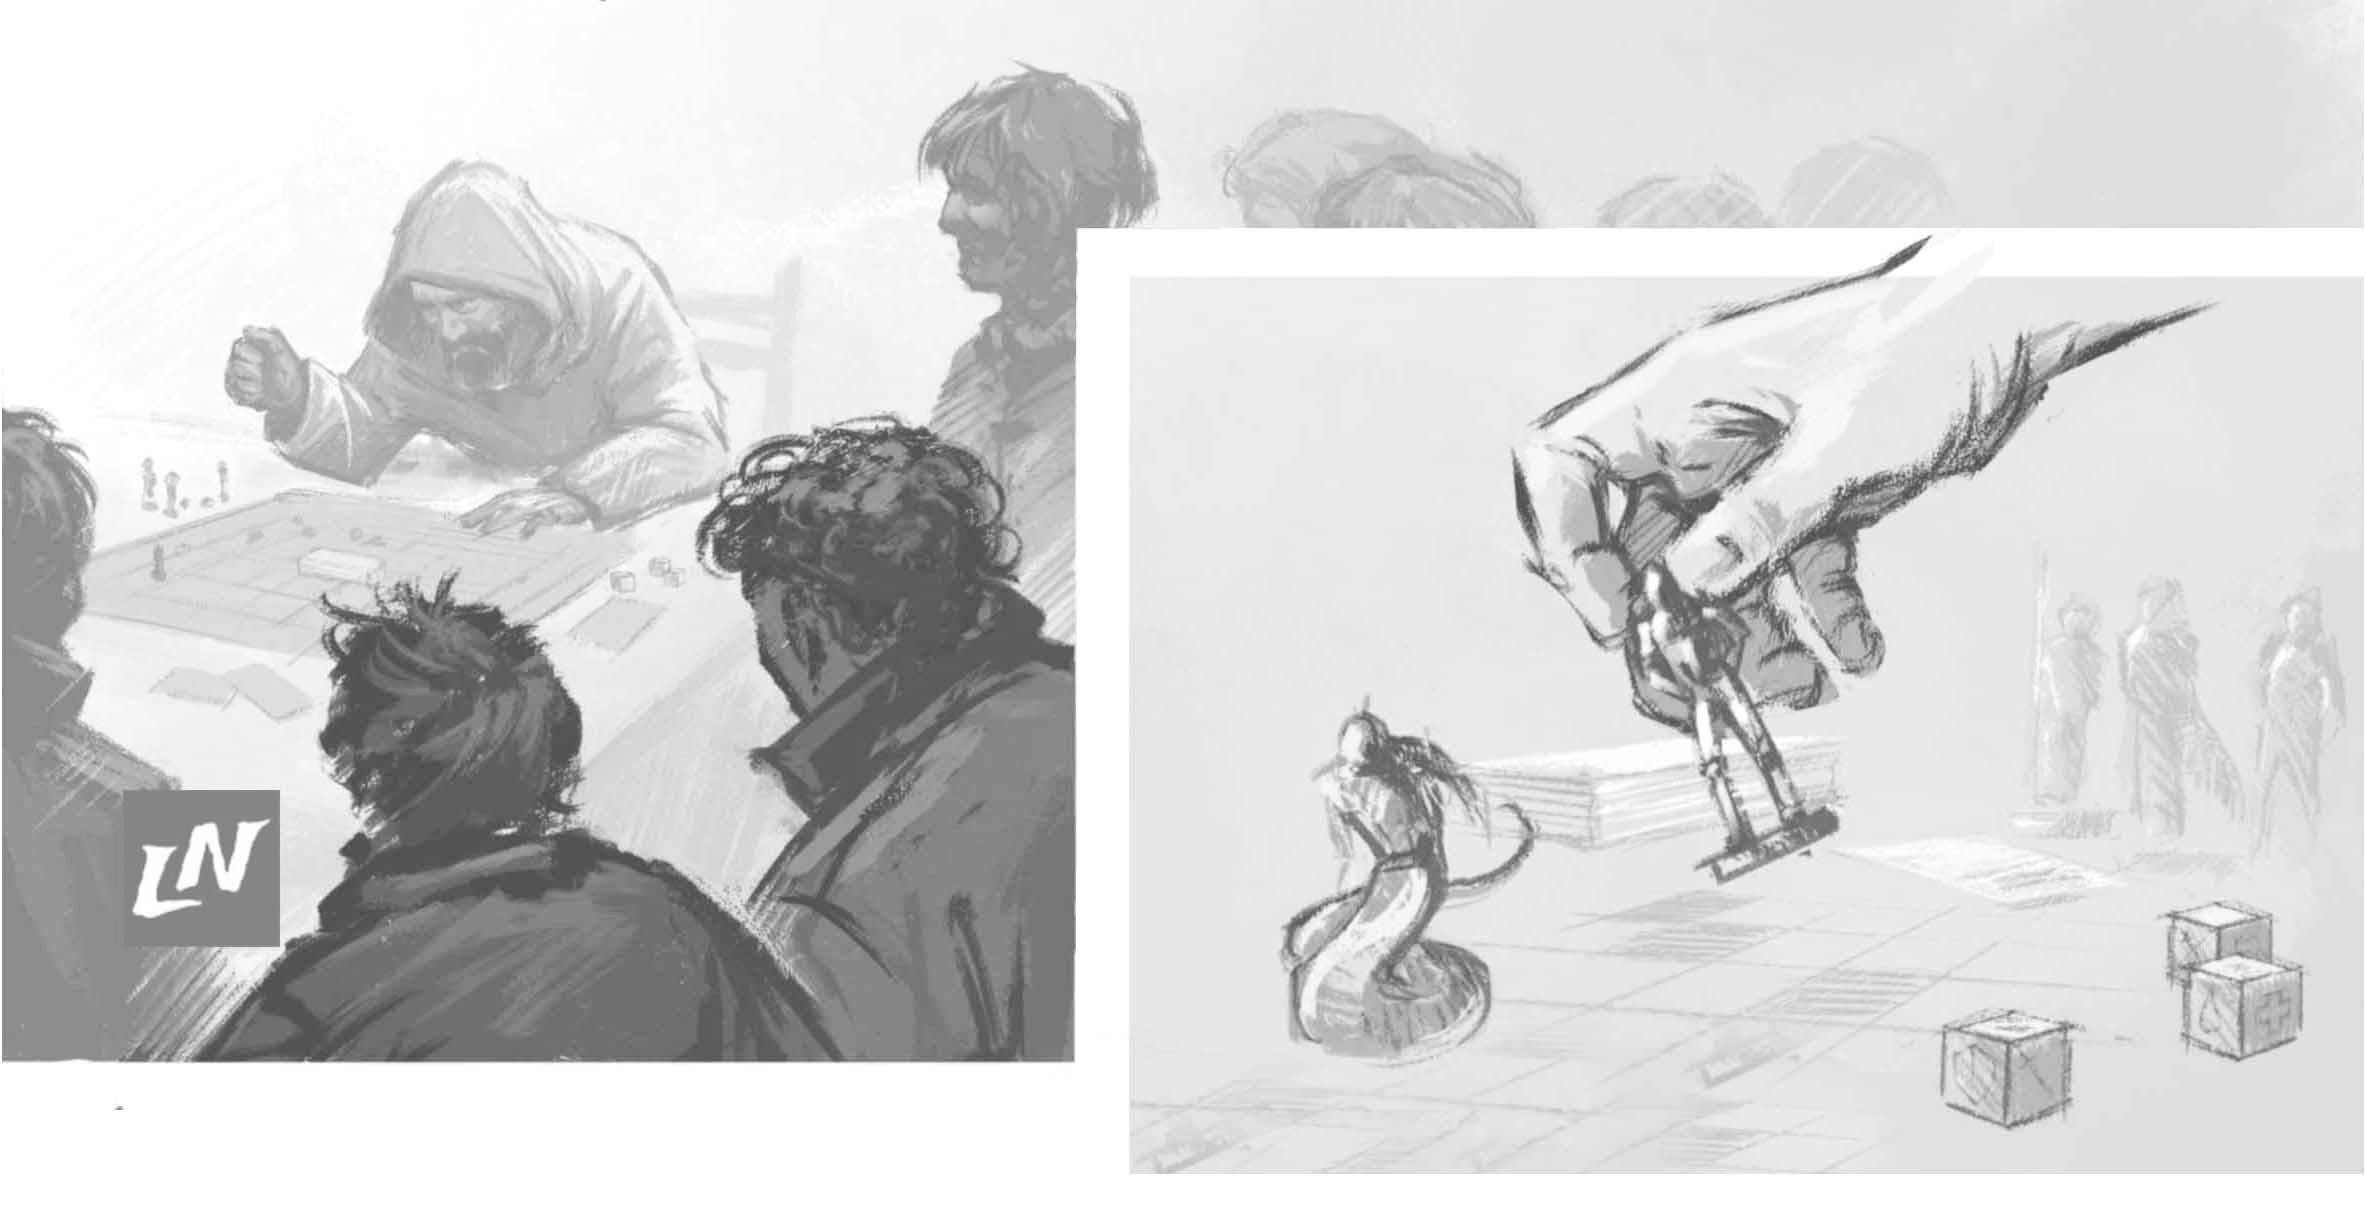
\includegraphics[width=0.999\textwidth]{./fig/tabletop.jpg}
\end{center}








%\vspace{2.0\baselineskip}
\clearpage %--------------------------------------------------------------------

\section*{Gold and Glory await the Brave Heroes}

\noindent
For the very young we have adventures like \texttt{Bitter Candy} where Lord Grapefruit is threatening to make all the sweets in the land taste like coffee. Play with your kids' favourite toys across half the house, or on a table using maps and meeples. Use grapes as the Villain's minions and have your kids eat their kills.

We also have the \texttt{Ominous Crown} example for slightly older children, or turn it into a small mini campaign for your brave new adult players. I hear wine, cheese, and crackers are excellent when you set out to rescue the Blacksmith's daughter.

New players should run their first new Hero through the \texttt{Dungeon of Testing}, where they will learn the basics in a non lethal environment.

\

\noindent
For a longer new player campaign we have \texttt{Return of Uchly Namen} where the newbies travel to Sleepy Cove chasing a "Heroes Wanted" ad. Goblins, bandits, monsters, from deep mine shafts to high towers. The Heroes travel the land and encounter a wide range of challenges, suitable to introduce the game in bite sized pieces.

When they have solved the mystery, now experienced almost-heroes, they can take on the \texttt{Dark Klan}, explore the \texttt{Deep Cave}, and go \texttt{Rescue Nurensachs}, in a mid range campaign arc. Also with completely new challenges.

\

\noindent
\texttt{Overlord Orvar} is an up and coming Dark Lord. He's set up shop close to Kleinshof and is preparing for his campaign of Death, Destruction, and Domination. Better stop him before it starts.

Then there is the ashen greyness spreading in the Eastern Mountains. \texttt{Edwin the Chromophobe} has awoken from his slumber and is slowly poisoning the world, his influence spreading from his Dread Tomb. The Heroes must delve into the dark depths to resolve the hiccup.

\

\noindent
At some point the Heroes should perhaps get Certified as Heroes of the Land? \texttt{Ottokar's Test Dungeon} provide those services for a bag of silver. Official Hero Certification is a racket, for sure, but many clueless middle management gnomes insist that they will only bring on Officially Certified Heroes for the task at hand.

Experienced Heroes can perhaps be hired for a dangerous mission to \texttt{Destroy the Altar} deep in the goblin warrens. This is not for the faint of heart nor weak of arm. And if they survive that they will be offered to \texttt{Turn off the Light}. How many Heroes does it take to unscrew a light bulb? How many will die in the process?

\

\noindent
Different kinds of challenges pop up in the \texttt{Goblin Destiny} campaign. We follow the GamGang bandits from when they have just moved in to when they finally fulfil their Destiny. Intended for experienced players, starting with noob goblin Heroes.


\vfill

\begin{center}
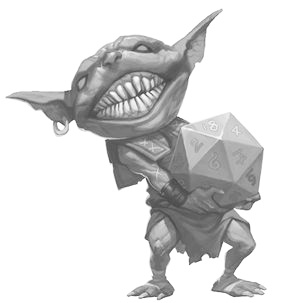
\includegraphics[height=45mm]{./fig/dicegoblin.jpg}
\end{center}







\clearpage %--------------------------------------------------------------------

\section*{Built for online gaming}

The rule set and campaign setting was explicitly built for online gaming. Most people want to play more than they can schedule. This is a way to make it happen.


\subsection*{A Virtual TableTop}

There are many choices available. Choose which one you and your players feel comfortable with. You don't need much support for special features. The basics are available in all common tools. Import maps from images. Import Hero and Monster tokens from images. Move tokens around on the map. All tools allow all players to access their Heroes on the map and move them around. The GM moves the monsters and NPCs.

Some tools have support for fog of war for exploration and sight, vision blocking for walls and objects, individual vision for each Hero, dynamic lighting and darkness, etc.
This adds a lot to the game, and allows for some interesting exploration and tactical gameplay not otherwise possible.
Great to have, but not necessary. You don't have it in a regular tabletop games, so you don't strictly need it.

Scripting is available in some tools. Helpful to build automation for common tasks and offload the old noggin from having to keep track of numbers and details.

\

We've used maptool through the years with good success. It has all the useful bells and whistles, and is open source and self hosted to boot. The scripting language is horrible, but I've managed to cobble together automation for all common tasks.


\subsection*{Voice chat}

So many options, but most of them suck donkey balls. Go with what you already like, but \emph{Don't} use teams, skype, webex, or other typical enterprise style conferencing tools. They are absolutely horrible. Conversation flow need under 100ms audio round trip.

Mumble is the best option we've found thus far. Great sound quality, best latency and jitter, and some other useful options. Open source and self hosted. Discord is simpler but has worse latency and quality. The old guard: teamspeak, ventrilo, etc probably still work. Hangouts, Zoom, et al. are generally worse and less reliable, but still better than teams et al.

\

\noindent
What the hell, just go with mumble! If you really can't be bothered to set it up, check out discord.


\subsection*{Sketching and writing}

Fun, and sometimes useful, to have a shared sketch table. Jarnal works but is very limited. There are a ton of tools on the web, with good and bad. Google docs work well for real time collaborative editing.


\vfill

\begin{center}
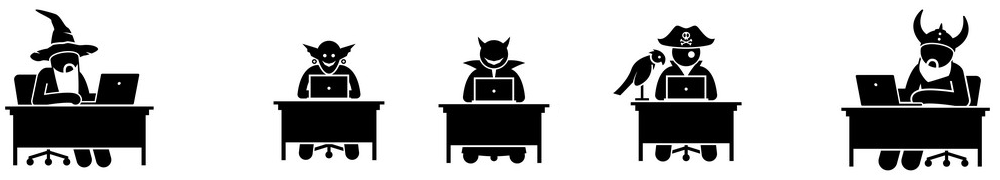
\includegraphics[width=0.99\textwidth]{./fig/online-warriors.png}
\end{center}








\clearpage %--------------------------------------------------------------------

\section*{Physical TableTop gaming}

The rule set is very flexible and easy to adapt to \emph{your} player group. Find a good trade off between speed and complexity. Start with the very small and basic rule set, then add interesting rules, skills, details, etc until you feel it's getting slow. Pick and choose as you go. Get rid of things you don't like and test new stuff that you find interesting. The game is exceptionally modular and very easy to tweak. There is an enormous space of interesting \emph{interactions} between all the optional parts, but very few \emph{interdependencies}, meaning you rarely need A to get B working.


\subsection*{Young Kids}

It really is super easy in the simplest basic version, without lots of extras. We've had successful games with kids as young as 5yo who have never played an adventure game, rpg, or tabletop before. Older kids have had no problem getting into the game. \emph{Keep it fun} and don't overload them.

Their small toys work perfectly well as Hero mini figs. You don't need a map grid, just use paper strips or strings to measure out movement and ranges. Use small pretty pearls and trinkets as hp and mana counters, etc. Be open minded and involve the kids, find something that works, and have fun. Adventure awaits, and it doesn't have to be complicated or involved in the beginning.

If they can count to 10, add and subtract a bit, they can play the game.


\subsection*{Battle maps, minis, terrain}

But even if quick sketches on a paper and some improvised tokens is enough to make the game work, it really looks cool with well built terrain, trees, houses, cavern floor, painted minis, and distinct markers, counters, and tokens.

The game is agnostic. Just use what you can scrounge up. A WH40k Genestealer serves perfectly well for a ClawRunner, and that old obscure lead figurine is a great MonsterX.
Or be as puritanical as you wish, excellent imagery awaits and the players will love it, but only if you want to.


\subsection*{Pen and paper, markers, tokens, counters}

A piece of paper with character and notes, together with some tokens and counters is enough to play full complexity, even if it will be a bit faster with vtt script automation.


\begin{figure}[b]
\centering
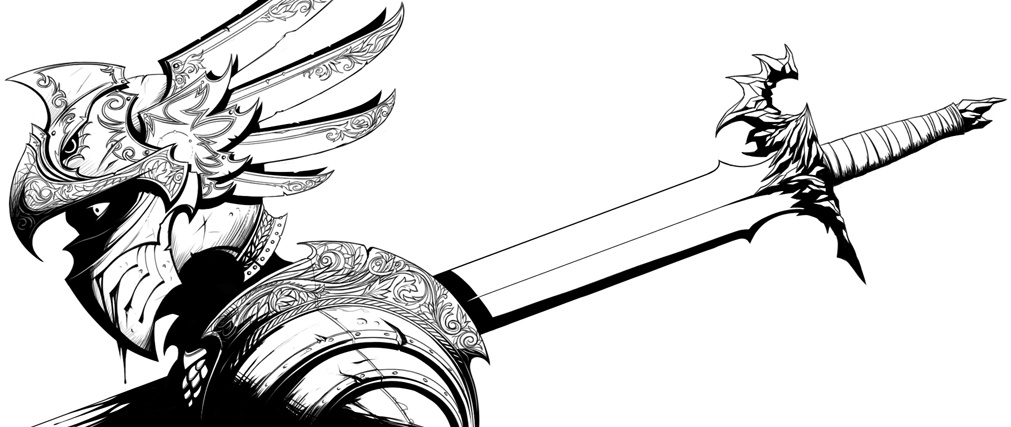
\includegraphics[width=120mm]{./fig/deadhero.jpg}
\end{figure}








\clearpage %--------------------------------------------------------------------


\section*{Kingsland}

The rules are setting agnostic and can be applied to most game worlds, from fantasy to contemporary to scifi. The default setting is Kingsland, a traditional mid fantasy world. Especially a tiny little corner of Kingsland, the small harbour town of Sleepy Cove and a few villages, forests, hills and mountains around it.

All the released adventures take place in this tiny region. The Heroes and general population don't know much more of the world than their immediate surroundings. Most have never travelled further than the neighbouring village, and have only heard stories and rumours of the greater Kingsland and whatever domains lie beyond.

The practical world is small and dense. It takes just a day or two between villages, and there are only a few of them. Two barons divide the land between them. This little lump of civilisation lives in general peace and quiet. As the campaigns and adventures play out the region will change. Baron Conq will topple Baron Pawa with his dastardly scheming. The SouthWood goblin bandits will be routed and the woods will be safer for a while, until GamGang moves in to claim the empty goblin cave. Overlord Orvar will leave a piece of well constructed prime dungeon real estate empty when he's killed. Who or what will move in to claim it?

Continue placing adventures in the region and keep fleshing out the villages, add npcs and stories. Make the region come alive and anchor it with players. This is a good way to make it feel real. Exploration, experience, memories, stories.



\vfill

\begin{center}
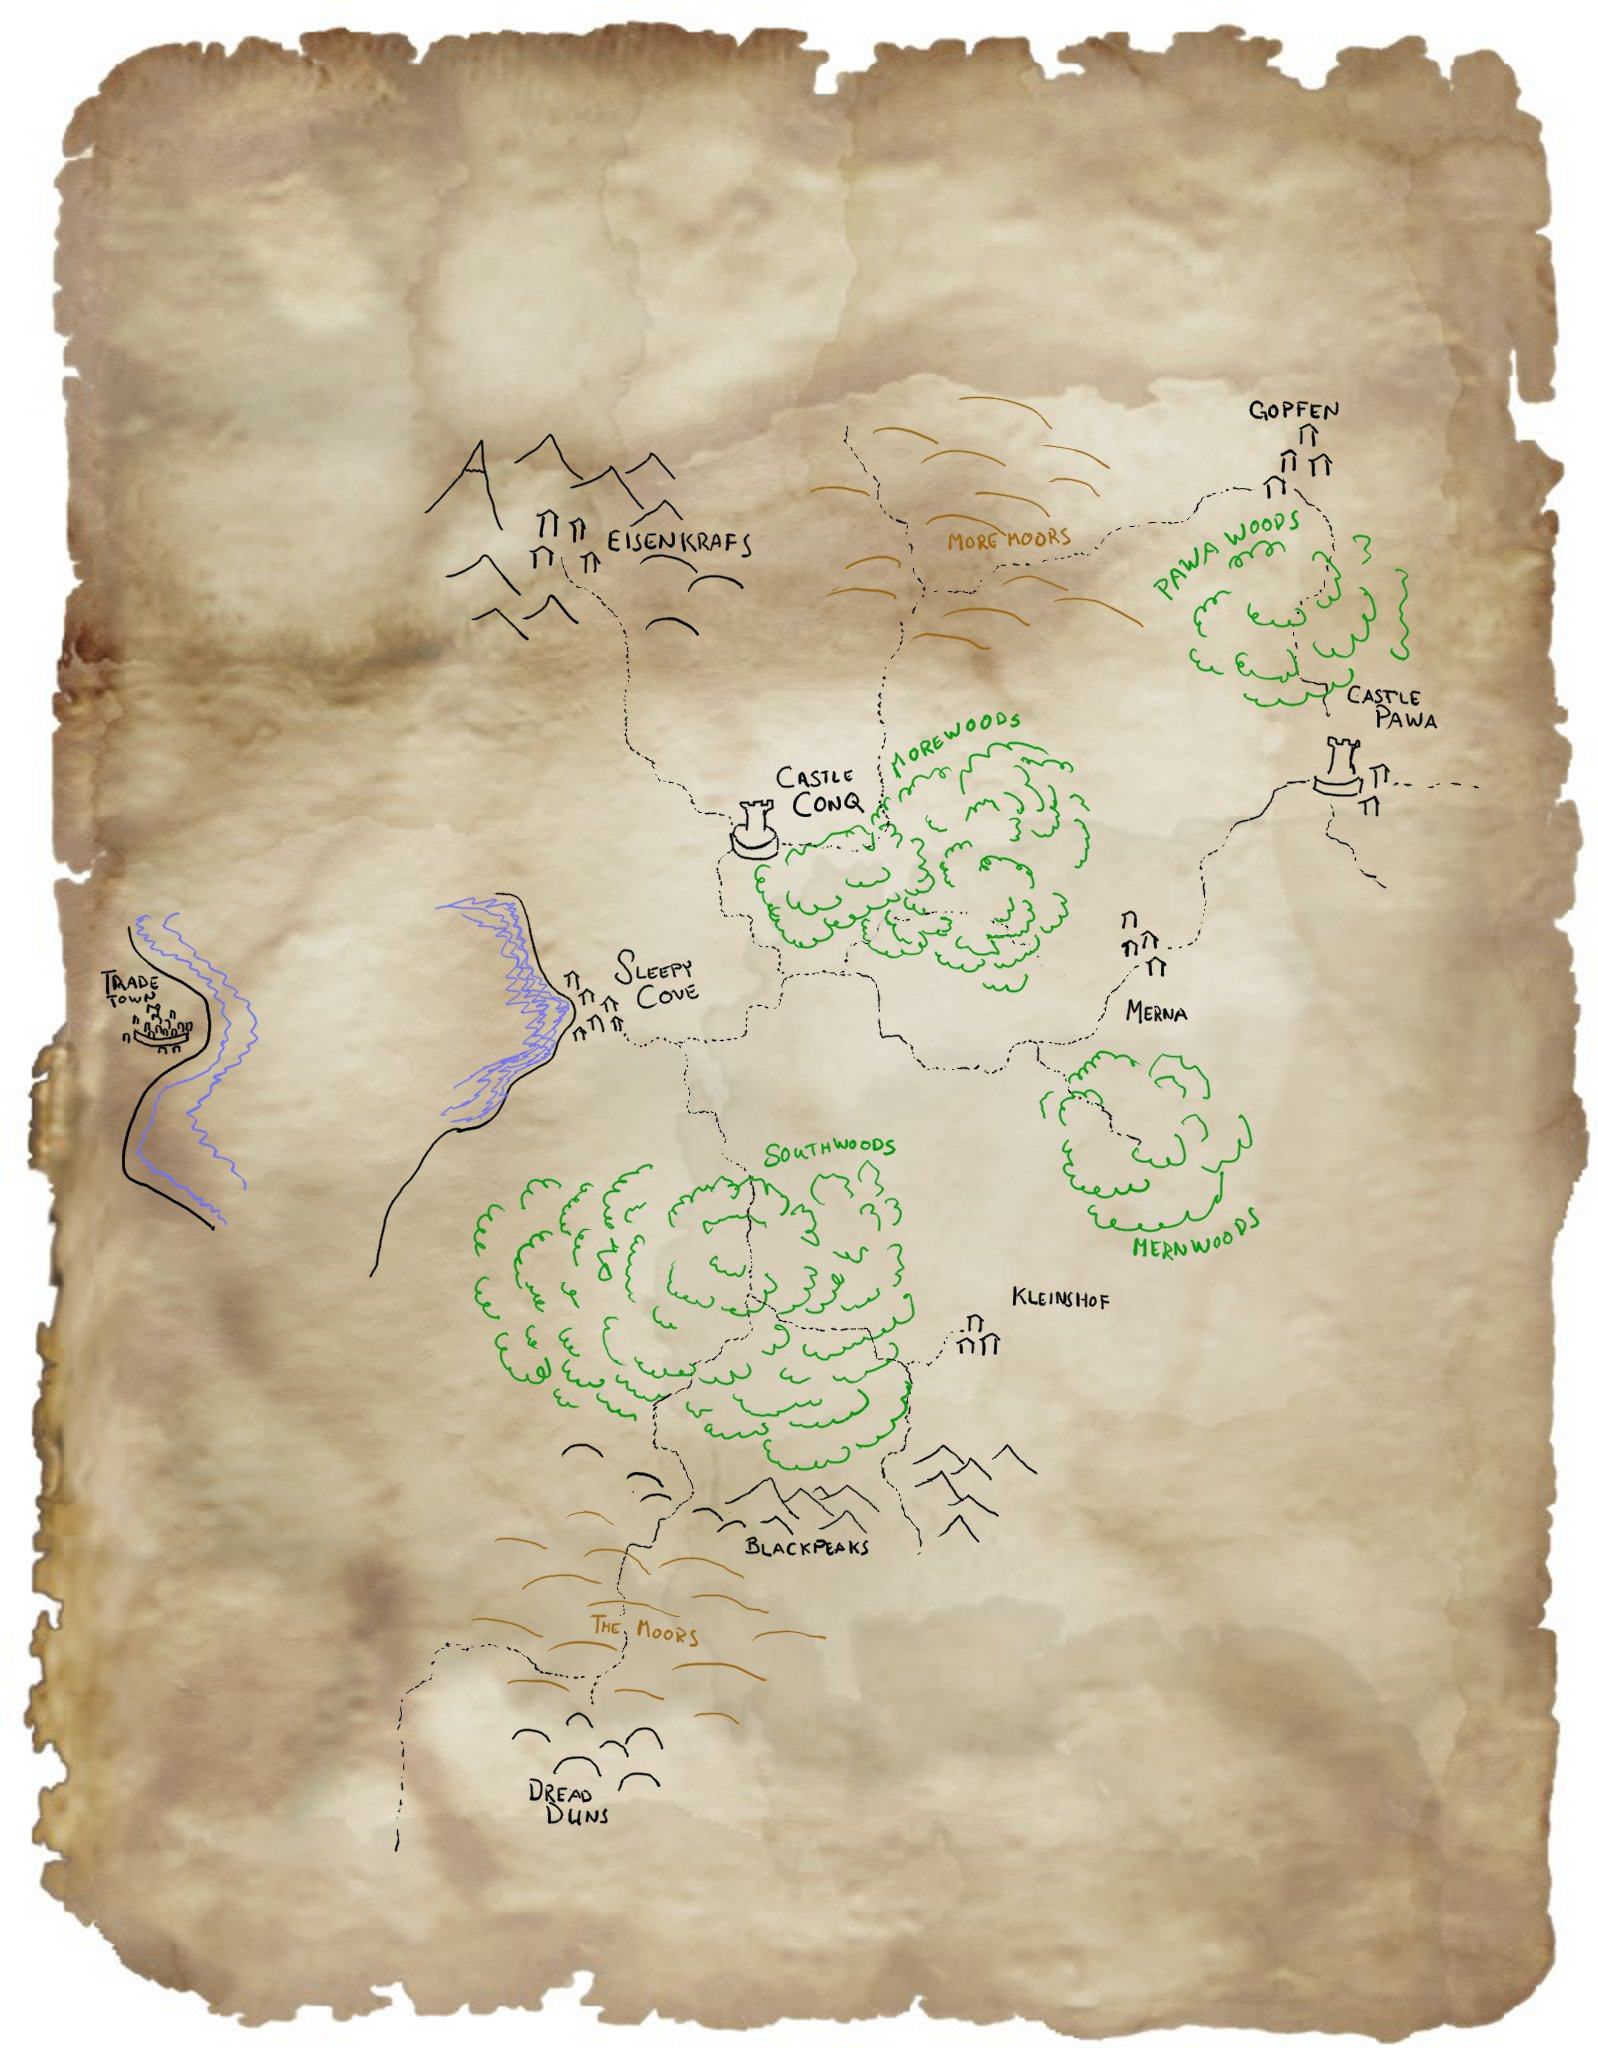
\includegraphics[height=130mm]{./map/region-roun-pc.jpg}
\end{center}


%\clearpage %--------------------------------------------------------------------
%
%\thispagestyle{empty}
%
%\begin{figure}[t]
%\centering
%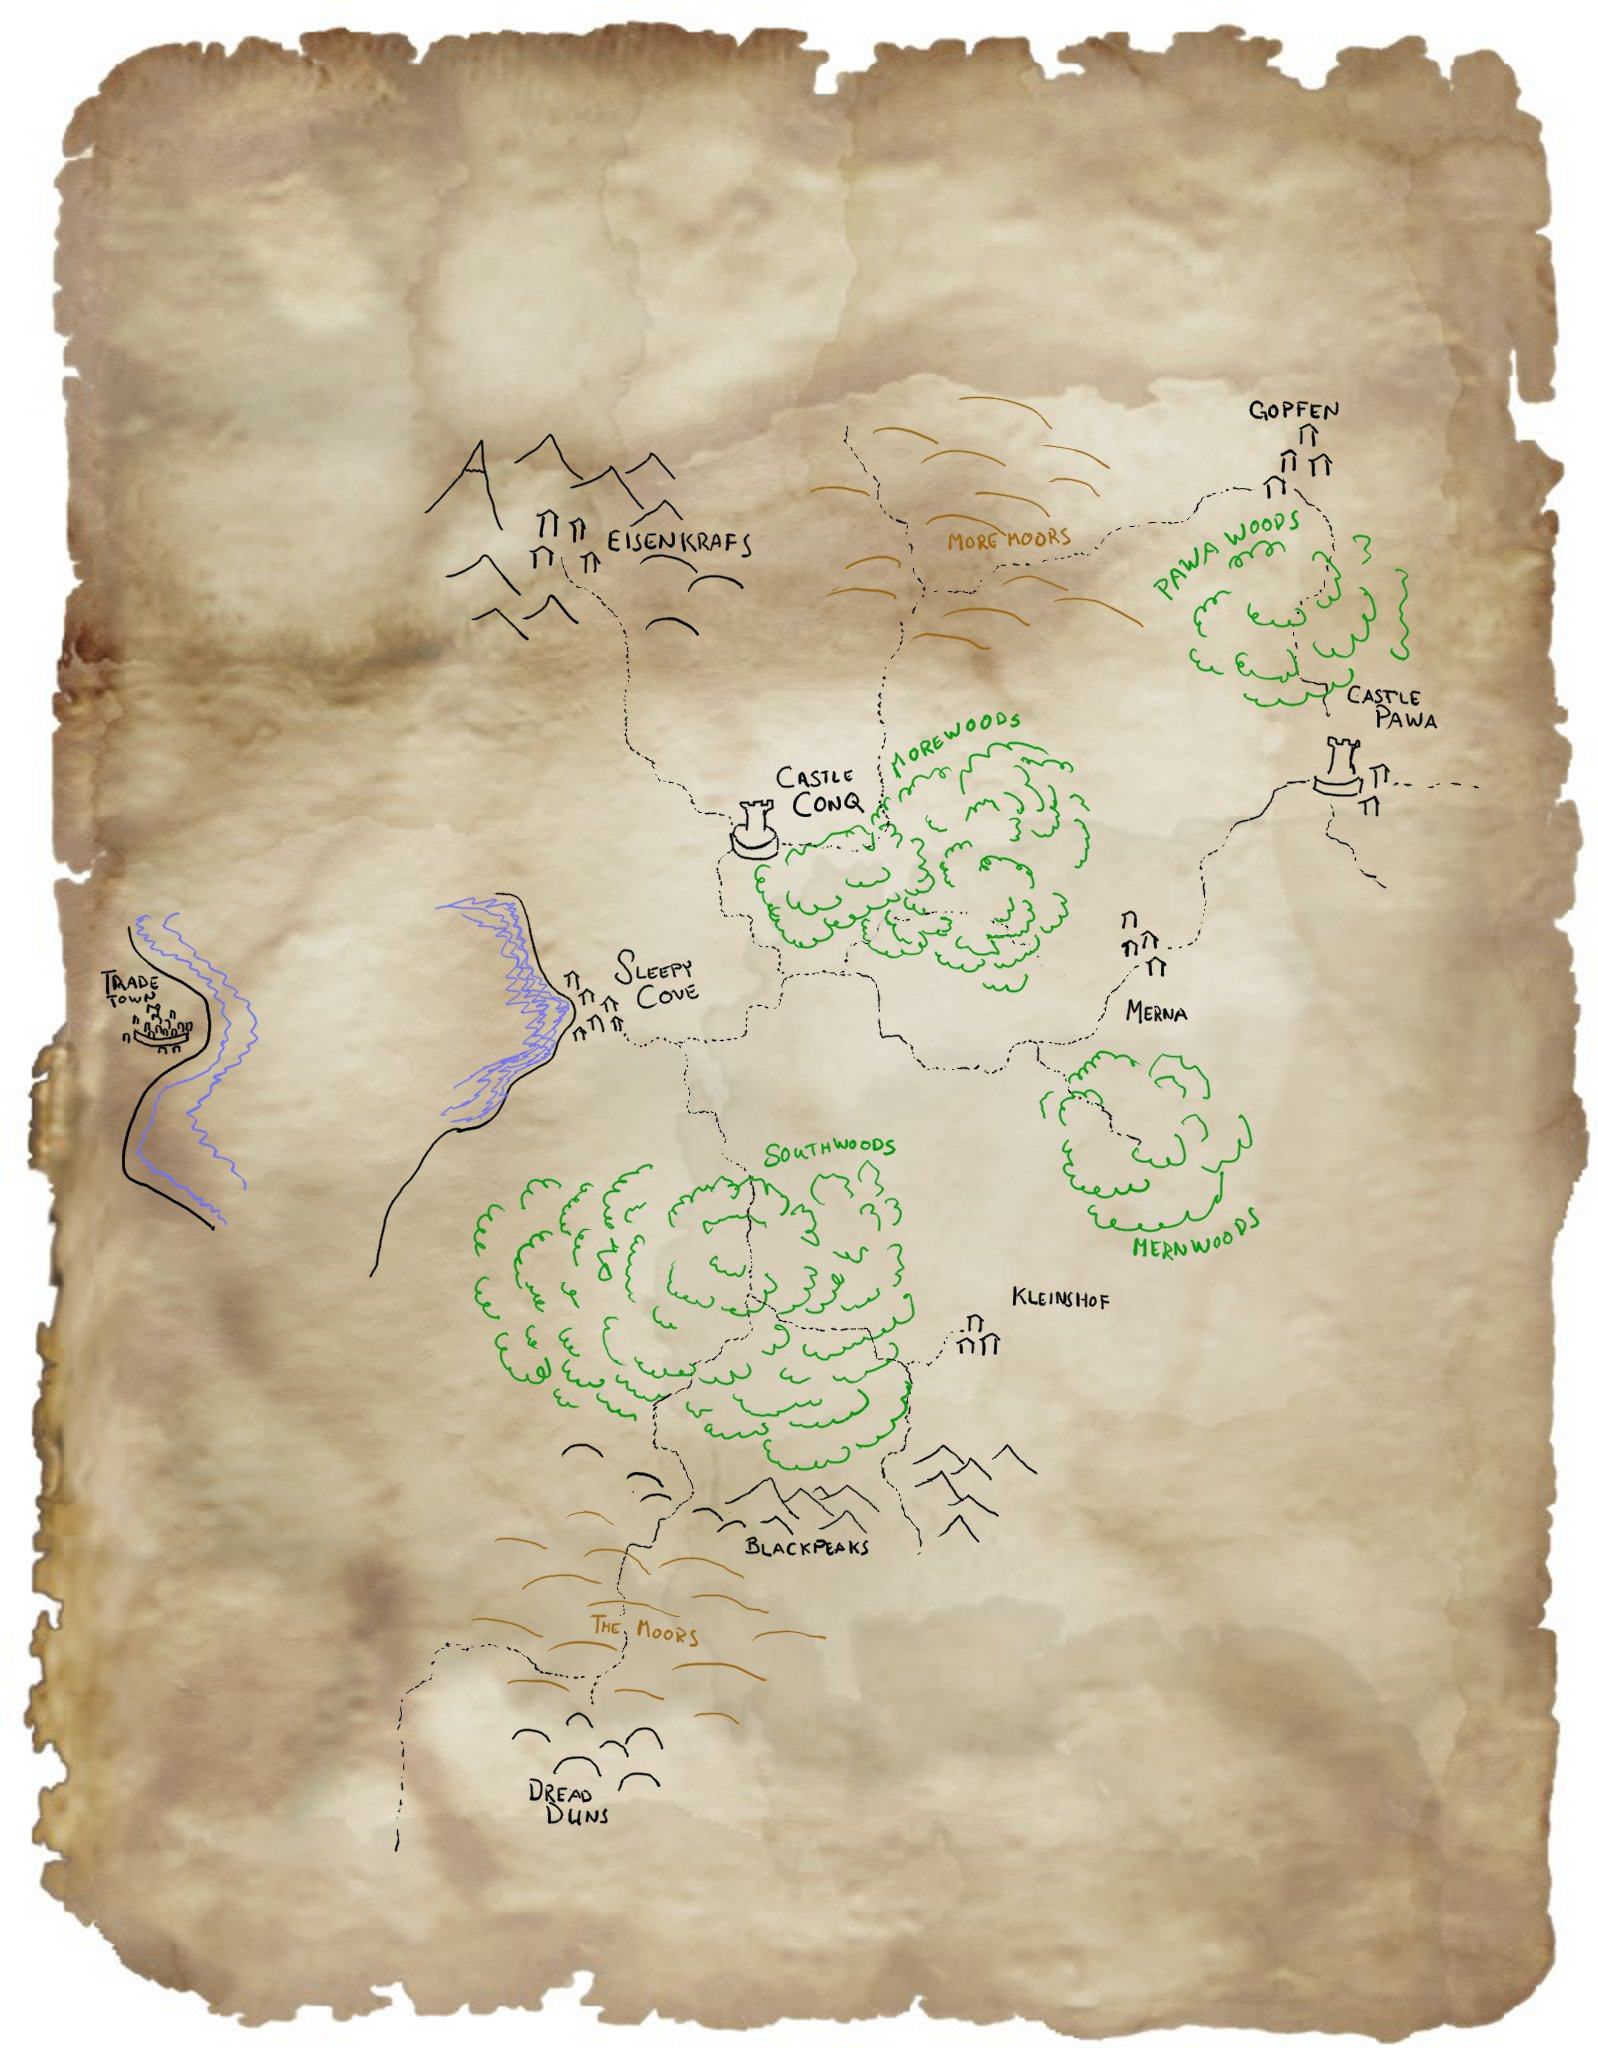
\includegraphics[width=0.999\textwidth]{./map/region-roun-pc.jpg}
%\end{figure}





%-------------------------------------------------------------------------------
\end{document}
